\documentclass[11pt,a4paper]{article}
%%%%%%%%%%%%%%%%%%%%%%%%% Credit %%%%%%%%%%%%%%%%%%%%%%%%

% template ini dibuat oleh martin.manullang@if.itera.ac.id untuk dipergunakan oleh seluruh sivitas akademik itera.

%%%%%%%%%%%%%%%%%%%%%%%%% PACKAGE starts HERE %%%%%%%%%%%%%%%%%%%%%%%%
\usepackage{graphicx}
\usepackage{caption}
\captionsetup[table]{name=Tabel}
\captionsetup[figure]{name=Gambar}
\usepackage{tabulary}
% \usepackage{amsmath}
\usepackage{fancyhdr}
% \usepackage{amssymb}
% \usepackage{amsthm}
\usepackage{placeins}
% \usepackage{amsfonts}
\usepackage{graphicx}
\usepackage[all]{xy}
\usepackage{tikz}
\usepackage{verbatim}
\usepackage[left=2cm,right=2cm,top=3cm,bottom=2.5cm]{geometry}
\usepackage{hyperref}
\hypersetup{
    colorlinks,
    linkcolor={red!50!black},
    citecolor={blue!50!black},
    urlcolor={blue!80!black}
}
\usepackage{libertine}
\usepackage{libertinust1math}
\usepackage[T1]{fontenc}
\usepackage{inconsolata}

\usepackage{caption}
\usepackage{subcaption}
\usepackage{multirow}
\usepackage{psfrag}
\usepackage[T1]{fontenc}
\usepackage[scaled]{beramono}
% Enable inserting code into the document
\usepackage{listings}
\usepackage{xcolor} 
% custom color & style for listing
\definecolor{codegreen}{rgb}{0,0.6,0}
\definecolor{codegray}{rgb}{0.5,0.5,0.5}
\definecolor{codepurple}{rgb}{0.58,0,0.82}
\definecolor{backcolour}{rgb}{0.95,0.95,0.92}
\lstdefinestyle{mystyle}{
	backgroundcolor=\color{backcolour},   
	commentstyle=\color{green},
	keywordstyle=\color{codegreen},
	numberstyle=\tiny\color{codegray},
	stringstyle=\color{codepurple},
	basicstyle=\ttfamily\footnotesize,
	breakatwhitespace=false,         
	breaklines=true,                 
	captionpos=b,                    
	keepspaces=true,                 
	numbers=left,                    
	numbersep=5pt,                  
	showspaces=false,                
	showstringspaces=false,
	showtabs=false,                  
	tabsize=2
}
\lstset{style=mystyle}
\renewcommand{\lstlistingname}{Kode}
%%%%%%%%%%%%%%%%%%%%%%%%% PACKAGE ends HERE %%%%%%%%%%%%%%%%%%%%%%%%


%%%%%%%%%%%%%%%%%%%%%%%%% Data Diri %%%%%%%%%%%%%%%%%%%%%%%%
\newcommand{\stuid}{120140225}
\newcommand{\student}{\textbf{Zointa Ras Bangun (\stuid{})}}
\newcommand{\course}{\textbf{Sistem Operasi RD (IF2223)}}
\newcommand{\assignment}{\textbf{2}} % tugas ke...

%%%%%%%%%%%%%%%%%%% using theorem style %%%%%%%%%%%%%%%%%%%%
\newtheorem{thm}{Theorem}
\newtheorem{lem}[thm]{Lemma}
\newtheorem{defn}[thm]{Definition}
\newtheorem{exa}[thm]{Example}
\newtheorem{rem}[thm]{Remark}
\newtheorem{coro}[thm]{Corollary}
\newtheorem{quest}{Question}[section]
%%%%%%%%%%%%%%%%%%%%%%%%%%%%%%%%%%%%%%%%
\usepackage{lipsum}%% a garbage package you don't need except to create examples.
\usepackage{fancyhdr}
\usepackage[ddmmyyyy]{datetime}
\pagestyle{fancy}
\lhead{Zointa Ras Bangun (120140225)}
\rhead{ \thepage}
\cfoot{\textbf{HandsOn 2 : Synchronisation and Deadlock}} % ini untuk judul tugas
\renewcommand{\headrulewidth}{0.4pt}
\renewcommand{\footrulewidth}{0.4pt}

%%%%%%%%%%%%%%  Shortcut for usual set of numbers  %%%%%%%%%%%

\newcommand{\N}{\mathbb{N}}
\newcommand{\Z}{\mathbb{Z}}
\newcommand{\Q}{\mathbb{Q}}
\newcommand{\R}{\mathbb{R}}
\newcommand{\C}{\mathbb{C}}
\setlength\headheight{14pt}

%%%%%%%%%%%%%%%%%%%%%%%%%%%%%%%%%%%%%%%%%%%%%%%%%%%%%%%555

\begin{document}
\thispagestyle{empty}
\begin{center}
	\includegraphics[scale = 0.15]{Figure/ifitera-header.png}
	\vspace{0.1cm}
\end{center}
\noindent
% change font family for header section only
%{\fontfamily{LinuxLibertineT-OsF}\large\selectfont 
{\large
\rule{17cm}{0.2cm}\\[0.3cm]
Nama: \student \hfill Tugas Ke: \assignment\\[0.1cm]
Mata Kuliah: \course \hfill Tanggal: \today\\
\rule{17cm}{0.05cm}
\vspace{0.1cm}
}


%%%%%%%%%%%%%%%%%%%%%%%%%%%%%%%%%%%%%%%%%%%%% BODY DOCUMENT %%%%%%%%%%%%%%%%%%%%%%%%%%%%%%%%%%%%%%%%%%%%%
\section{Tujuan HandsOn}
    HandsOn 2 bertujuan untuk memahami - sistem sinkronisasi dan permasalahan yang ada, Memahami solusi dalam menangani *critical section*, Memahami implementasi dari:
    - `join` menggunakan semaphores
- Binary Semaphores
- Producer Consumer
- Reader / Writer Locks
- Dining Philosophers
    
\section{\textbf{Fork}/Join}
\subsection{Source Code}
    \begin{lstlisting}[language=C,label={labelkode}]
    class SynthiaDataset(Dataset):
    #include <stdio.h>
    #include <stdlib.h>
    #include <pthread.h>
    #include <unistd.h>

    #include "common.h"
    #include "common_threads.h"

    #ifdef linux
    #include <semaphore.h>
    #elif APPLE
    #include "zemaphore.h"
    #endif

    sem_t s;

    void *child(void *arg) {
        sleep(2);
        printf("child\n");
        Sem_post(&s); // signal here: child is done
        return NULL;
    }

    int main(int argc, char *argv[]) {
        Sem_init(&s, 0); 
        printf("parent: begin\n");
        pthread_t c;
        Pthread_create(&c, NULL, child, NULL);
        Sem_wait(&s); // wait here for child
        printf("parent: end\n");
        return 0;
    }
    \end{lstlisting}
\subsection{\textbf{Output}}
    Berikut contoh output dari terminal yang saya buat :
    
\begin{figure}[h]
    \centering
    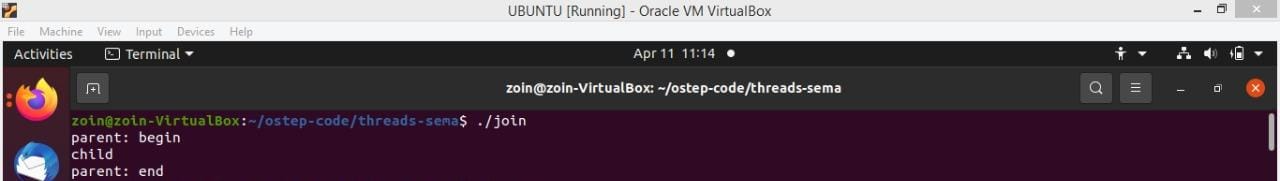
\includegraphics[scale = 0.4]{Figure/gambar/join_6_11zon.png}
    \caption{Tampilan \textit{fork}/join }
    \label{fig:join}
\end{figure}

\subsection{\textbf{Penjelasan}}
    Semaphore bisa dikatakan sebuah struktur data komputer yang berguna dalam sinkronisasi proses dan berfungsi dalam memerintsh jalannya proses suatu program. contohnya adalah suatu \textit{thread} menunggu \textit{list} supaya \textit{list} tersebut berisi atau tidak kosong. Dari kondisi tersebut, semaphore tadi akan di definisikan dan di inisiasi menjadi 0 oleh Sem init. Maksud dari proses tersebut ialah semaphore akan dibagi antara threads pada proses yang sama. Kemudian apabila pembuatan thread sudah selesai akan dilanjutkan pemanggilan fungsi child semaphore yang akan melakukan sinyal bahwa proses child sudah selesai dan mulai me-return. Apabila child sudah selesai, maka semaphore akan melanjutkannya dan mengeluarkan output "parent : end".
    
    
    
\section{\textbf{Binary Semaphores}}
\subsection{Source Code }
    \begin{lstlisting}[language=C,label={labelkode}]
    class SynthiaDataset(Dataset):
    #include <stdio.h>
    #include <stdlib.h>
    #include <pthread.h>
    #include <unistd.h>

    #include "common.h"
    #include "common_threads.h"

    #ifdef linux
    #include <semaphore.h>
    #elif APPLE
    #include "zemaphore.h"
    #endif

    sem_t mutex;
    volatile int counter = 0;

    void *child(void *arg) {
        int i;
        for (i = 0; i < 10000000; i++) {
	    Sem_wait(&mutex);
	    counter++;
	    Sem_post(&mutex);
        }
        return NULL;
    }

    int main(int argc, char *argv[]) {
        Sem_init(&mutex, 1); 
        pthread_t c1, c2;
        Pthread_create(&c1, NULL, child, NULL);
        Pthread_create(&c2, NULL, child, NULL);
        Pthread_join(c1, NULL);
        Pthread_join(c2, NULL);
        printf("result: %d (should be 20000000)\n", counter);
        return 0;
    }
    \end{lstlisting}
\subsection{\textbf{Output}}
    Berikut contoh output dari terminal yang saya buat :
    
    \begin{figure}[h]
        \centering
        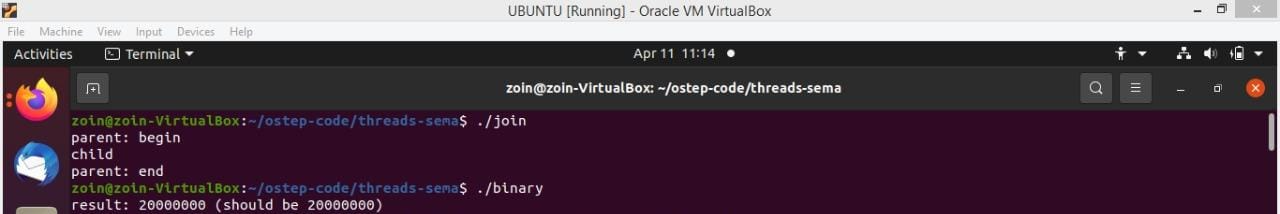
\includegraphics[scale = 0.4]{Figure/gambar/binary_1_11zon.png}
        \caption{Tampilan \textit{Binary}}
        \label{fig:tut2_1}
    \end{figure}
    
\subsection{Penjelasan \textit{Binary Semaphores}}
    pada kode diatas mendefinisikan dan menginisialisasikan semaphore mutex dengan value sebesar 1. lalu dibuat lah thread yang berinisial c1 dan c2 berguna dalam menjalan kan child. selanjutnya, akan dilakukan penginsialisasian pada perulangan sampai nilai tersebut kurang dari 1000000 yang mana akan menjalankan \textit{sem wait} dan di saat itu juga \textit{value} akan berkurang dan mulai dilakukan \textit{critical section}. akan ada penambahan nilai counter yang kemudian semaphore memproses calling dengan menambah value dari semaphore
    
\section{\textbf{Producer/Consumer}}
\subsection{\textbf{Source Code}}    
    \begin{lstlisting}[language=Python,label={labelkode}]
    
    class SynthiaDataset(Dataset):
    #include <stdio.h>
    #include <unistd.h>
    #include <assert.h>
    #include <pthread.h>
    #include <stdlib.h>

    #include "comm#include <stdio.h>
#include <unistd.h>
#include <assert.h>
#include <pthread.h>
#include <stdlib.h>

#include "common.h"
#include "common_threads.h"

#ifdef linux
#include <semaphore.h>
#elif __APPLE__
#include "zemaphore.h"
#endif

int max;
int loops;
int *buffer;

int use  = 0;
int fill = 0;

sem_t empty;
sem_t full;
sem_t mutex;

#define CMAX (10)
int consumers = 1;

void do_fill(int value) {
    buffer[fill] = value;
    fill++;
    if (fill == max)
	fill = 0;
}

int do_get() {
    int tmp = buffer[use];
    use++;
    if (use == max)
	use = 0;
    return tmp;
}

void *producer(void *arg) {
    int i;
    for (i = 0; i < loops; i++) {
	Sem_wait(&empty);
	Sem_wait(&mutex);
	do_fill(i);
	Sem_post(&mutex);
	Sem_post(&full);
    }

    // end case
    for (i = 0; i < consumers; i++) {
	Sem_wait(&empty);
	Sem_wait(&mutex);
	do_fill(-1);
	Sem_post(&mutex);
	Sem_post(&full);
    }

    return NULL;
}
                                                                               
void *consumer(void *arg) {
    int tmp = 0;
    while (tmp != -1) {
	Sem_wait(&full);
	Sem_wait(&mutex);
	tmp = do_get();
	Sem_post(&mutex);
	Sem_post(&empty);
	printf("%lld %d\n", (long long int) arg, tmp);
    }
    return NULL;
}

int main(int argc, char *argv[]) {
    if (argc != 4) {
	fprintf(stderr, "usage: %s <buffersize> <loops> <consumers>\n", argv[0]);
	exit(1);
    }
    max   = atoi(argv[1]);
    loops = atoi(argv[2]);
    consumers = atoi(argv[3]);
    assert(consumers <= CMAX);

    buffer = (int *) malloc(max * sizeof(int));
    assert(buffer != NULL);
    int i;
    for (i = 0; i < max; i++) {
	buffer[i] = 0;
    }

    Sem_init(&empty, max); // max are empty 
    Sem_init(&full, 0);    // 0 are full
    Sem_init(&mutex, 1);   // mutex

    pthread_t pid, cid[CMAX];
    Pthread_create(&pid, NULL, producer, NULL); 
    for (i = 0; i < consumers; i++) {
	Pthread_create(&cid[i], NULL, consumer, (void *) (long long int) i); 
    }
    Pthread_join(pid, NULL); 
    for (i = 0; i < consumers; i++) {
	Pthread_join(cid[i], NULL); 
    }
    return 0;
}
    \end{lstlisting}

\newpage   
\subsection{\textbf{Output}}
    Berikut contoh output dari terminal yang saya buat :
    
\begin{figure}[h]
	\centering
	\begin{subfigure}[b]{0.4\textwidth}
		\centering
		\def\svgwidth{\columnwidth}
		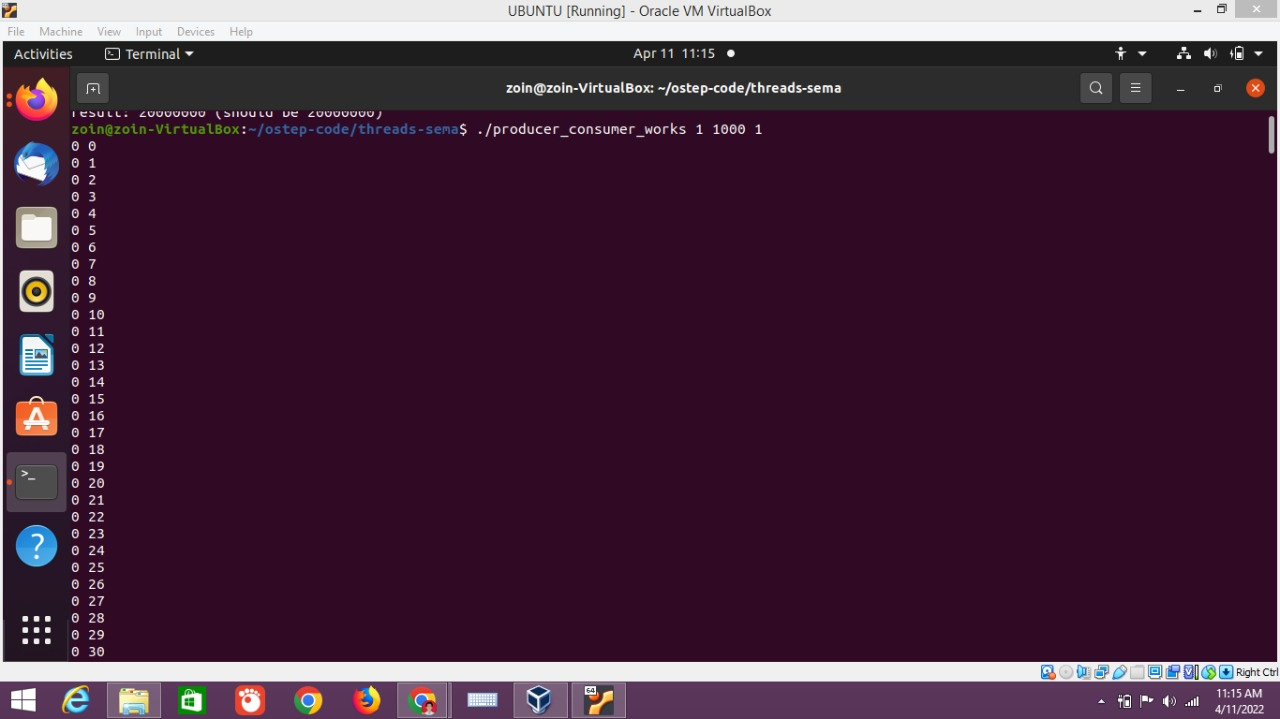
\includegraphics[width=1\textwidth]{Figure/gambar/producer 1_10_11zon.png}
		\caption{Augment Result 1}
		\label{fig:aug-1}
	\end{subfigure}
	\qquad %add desired spacing between images, e. g. ~, \quad, \qquad, \hfill etc. 
	%(or a blank line to force the subfigure onto a new line)
	\begin{subfigure}[b]{0.4\textwidth}
		\centering
		\def\svgwidth{\columnwidth}
		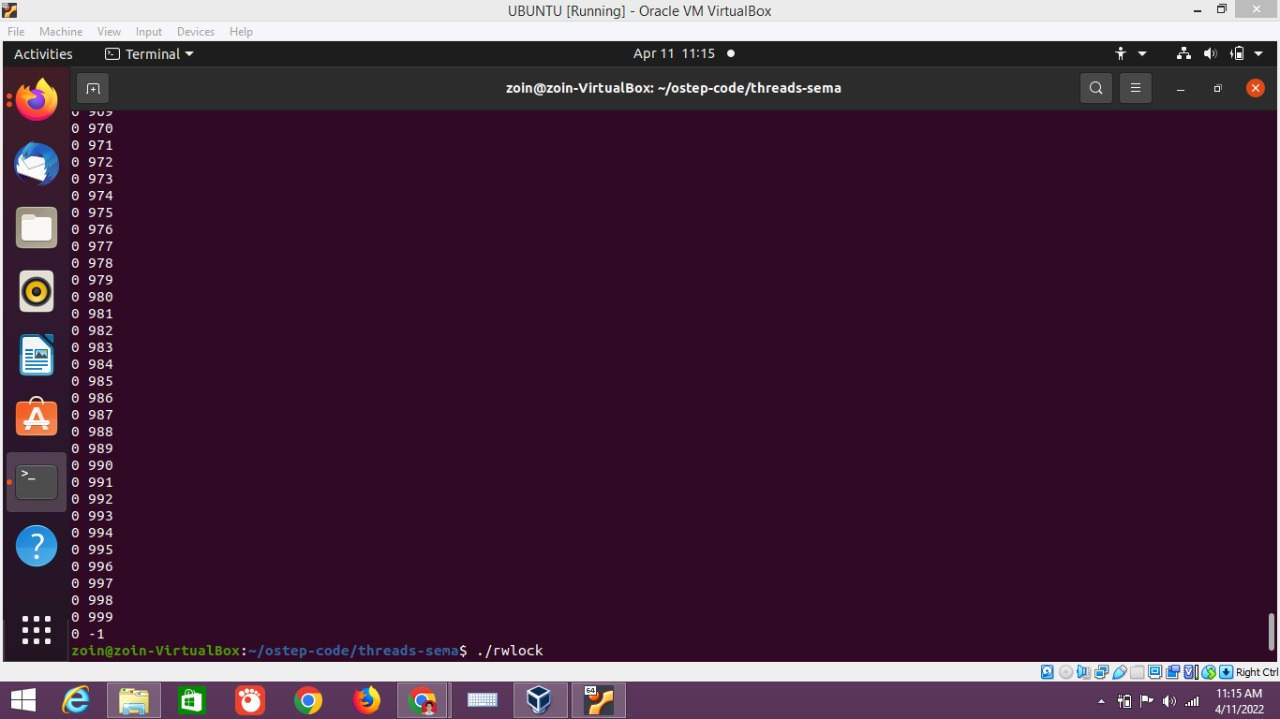
\includegraphics[width=1\textwidth]{Figure/gambar/producer 2_11_11zon.png}
		\caption{Augment Result 2}
		\label{fig:aug-2}
	\end{subfigure}
	\caption{Screenshot Percobaan}\label{fig:aug}
\end{figure}

\subsection{\textbf{Penjelasan Producer Consumer}}
Implementasi Producer/Consumer disebut bounded buffer. Isi program tersebut ialah memanggil, mengurangi, menghalangi konsumer, dan menunggu thread lain agar dapat memanggil
Sem post saat terjadi full. Selanjutnya, program akan memulai fungsi procedure yang berguna dalam memanggil Sem wait(empty) dan Sem post(mutex). Pada fungsi procedur juga menjalankan terus sampai empty tadi menjadi max. Producer akan melakukan pengisian dengan fungsi do fill di entry pertama buffer setelah empty berkurang hingga mencapai nilai 0. Berikutnya, producer akan terus berjalan sampai suatu saat nanti memanggil Sem post(mutex) dan Sem post(full) yang mana akan mengganti nilai value full dari nilai -1 menjadi 0. Sehingga, Consumer akan melakukan fungsi looping ulang dan memblok dengan value empty semaphore
bernilai kosong.

\section{\textbf{Reader or Writer Locks}}
\subsection{\textbf{Source Code}}
    \begin{lstlisting}[language=C++, label={labelkode}]
#include <stdio.h>
#include <stdlib.h>
#include <pthread.h>
#include <unistd.h>

#include "common.h"
#include "common_threads.h"

#ifdef linux
#include <semaphore.h>
#elif __APPLE__
#include "zemaphore.h"
#endif

typedef struct _rwlock_t {
    sem_t writelock;
    sem_t lock;
    int readers;
} rwlock_t;

void rwlock_init(rwlock_t *lock) {
    lock->readers = 0;
    Sem_init(&lock->lock, 1); 
    Sem_init(&lock->writelock, 1); 
}

void rwlock_acquire_readlock(rwlock_t *lock) {
    Sem_wait(&lock->lock);
    lock->readers++;
    if (lock->readers == 1)
	Sem_wait(&lock->writelock);
    Sem_post(&lock->lock);
}

void rwlock_release_readlock(rwlock_t *lock) {
    Sem_wait(&lock->lock);
    lock->readers--;
    if (lock->readers == 0)
	Sem_post(&lock->writelock);
    Sem_post(&lock->lock);
}

void rwlock_acquire_writelock(rwlock_t *lock) {
    Sem_wait(&lock->writelock);
}

void rwlock_release_writelock(rwlock_t *lock) {
    Sem_post(&lock->writelock);
}

int read_loops;
int write_loops;
int counter = 0;

rwlock_t mutex;

void *reader(void *arg) {
    int i;
    int local = 0;
    for (i = 0; i < read_loops; i++) {
	rwlock_acquire_readlock(&mutex);
	local = counter;
	rwlock_release_readlock(&mutex);
	printf("read %d\n", local);
    }
    printf("read done: %d\n", local);
    return NULL;
}

void *writer(void *arg) {
    int i;
    for (i = 0; i < write_loops; i++) {
	rwlock_acquire_writelock(&mutex);
	counter++;
	rwlock_release_writelock(&mutex);
    }
    printf("write done\n");
    return NULL;
}

int main(int argc, char *argv[]) {
    if (argc != 3) {
	fprintf(stderr, "usage: rwlock readloops writeloops\n");
	exit(1);
    }
    read_loops = atoi(argv[1]);
    write_loops = atoi(argv[2]);
    
    rwlock_init(&mutex); 
    pthread_t c1, c2;
    Pthread_create(&c1, NULL, reader, NULL);
    Pthread_create(&c2, NULL, writer, NULL);
    Pthread_join(c1, NULL);
    Pthread_join(c2, NULL);
    printf("all done\n");
    return 0;
}
    \end{lstlisting}
\subsection{\textbf{Output}}
    Berikut hasil percobaan yang saya buat pada terminal :
    
    \begin{figure}[h]
        \centering
        
\includegraphics[scale = 0.5]{Figure/gambar/rwlock_12_11zon.png}
        \caption{Membuat shell script di nano}
        \label{fig:asg6_1}
    \end{figure}

\subsection{\textbf{Penjelasan Reader/writer Locks}}
   Secara umumnya, semaphore writelock untuk memastikan hanya satu writer saja yang mendapatkan lock dan memperbaruistruktur datanya dengan masuknya ke critical section. Kondisi ketika lock didapatkan, reader yang pertama akan mendapatkan lock tersebut dan mulai menambahkan variabel pembaca agar dapat melacak berapa pembaca yang ada saat ini pada struktur data. Perlu diperhatikan bahwa rwlock acquire readlock terjadi saat pembaca ke-1 mendapatkan lock dan writelock dengan memanggil Sem wait pada saat semaphore writelock yang akan dilepaskan lock-nya saat memanggil Sem post. \\\\
   Write process dan read process saling berpasangan hal ini akan membuat perubahan terutama pada proses di overhead karena sekalinya write process tertahan atau menunggu maka read process juga tertahan yang membuat bukan mempercepat, tapi memperlambat.

\newpage   
\section{\textbf{Dining Philosophers}}
\subsection{\textbf{Deadlock}}
BDining Philosophers adalah salah satu problem yang kemudian ditemukan Dijkstra yaitu idenya yang berupa logika 5 filsuf di sebuah meja makan berbentuk lingkaran, kemudian membuat perumpamaan para filsuf tersebut akan mengambil garpu di sisi kanan dan kirinya. Hal yang menjadi permasalahan adalah ketika dua filsuf yang berdampingan namun mengambil garpu yang sama. Oleh karena itu diperlukan fungsi bantu yang disebut left dan right. Kondisi ketika salah satu philosopher merunjuk pada suatu arah, ia akan mengajak bagian yang lain untuk mengatasi persoalan pada bagian lain

\subsubsection{\textbf{Source code}}
\begin{lstlisting}[language=C, caption= Source code,label={labelkode}]
    
    class SynthiaDataset(Dataset):

    #include <stdio.h>
    #include <stdlib.h>
    #include <pthread.h>

    #include "common.h"
    #include "common_threads.h"

    #ifdef linux
    #include <semaphore.h>
    #elif APPLE
    #include "zemaphore.h"
    #endif

    typedef struct {
        int num_loops;
        int thread_id;
    } arg_t;

    sem_t forks[5];
    sem_t print_lock;

    void space(int s) {
        Sem_wait(&print_lock);
        int i;
        for (i = 0; i < s * 10; i++)
	    printf(" ");
    }

    void space_end() {
        Sem_post(&print_lock);
    }

    int left(int p)  {
        return p;
    }

    int right(int p) {
        return (p + 1) % 5;
    }

    void get_forks(int p) {
        space(p); printf("%d: try %d\n", p, left(p)); space_end();
        Sem_wait(&forks[left(p)]);
        space(p); printf("%d: try %d\n", p, right(p)); space_end();
        Sem_wait(&forks[right(p)]);
    }

    void put_forks(int p) {
        Sem_post(&forks[left(p)]);
        Sem_post(&forks[right(p)]);
    }

    void think() {
        return;
    }

    void eat() {
        return;
    }

    void *philosopher(void *arg) {
        arg_t *args = (arg_t *) arg;

        space(args->thread_id); printf("%d: start\n", args->thread_id); space_end();

        int i;
        for (i = 0; i < args->num_loops; i++) {
	    space(args->thread_id); printf("%d: think\n", args->thread_id); space_end();
	    think();
	    get_forks(args->thread_id);
	    space(args->thread_id); printf("%d: eat\n", args->thread_id); space_end();
	    eat();
	    put_forks(args->thread_id);
	    space(args->thread_id); printf("%d: done\n", args->thread_id); space_end();
        }
        return NULL;
    }
                                                                             
    int main(int argc, char *argv[]) {
        if (argc != 2) {
	    fprintf(stderr, "usage: dining_philosophers <num_loops>\n");
	    exit(1);
        }
        printf("dining: started\n");
    
        int i;
        for (i = 0; i < 5; i++) 
	    Sem_init(&forks[i], 1);
        Sem_init(&print_lock, 1);

        pthread_t p[5];
        arg_t a[5];
        for (i = 0; i < 5; i++) {
	    a[i].num_loops = atoi(argv[1]);
	    a[i].thread_id = i;
	    Pthread_create(&p[i], NULL, philosopher, &a[i]);
        }

        for (i = 0; i < 5; i++) 
	    Pthread_join(p[i], NULL); 

        printf("dining: finished\n");
        return 0;
    }
    \end{lstlisting}
    
\newpage   
\subsubsection{\textbf{Output Print Deadlock}}
    \begin{figure}[h]
    \centering
    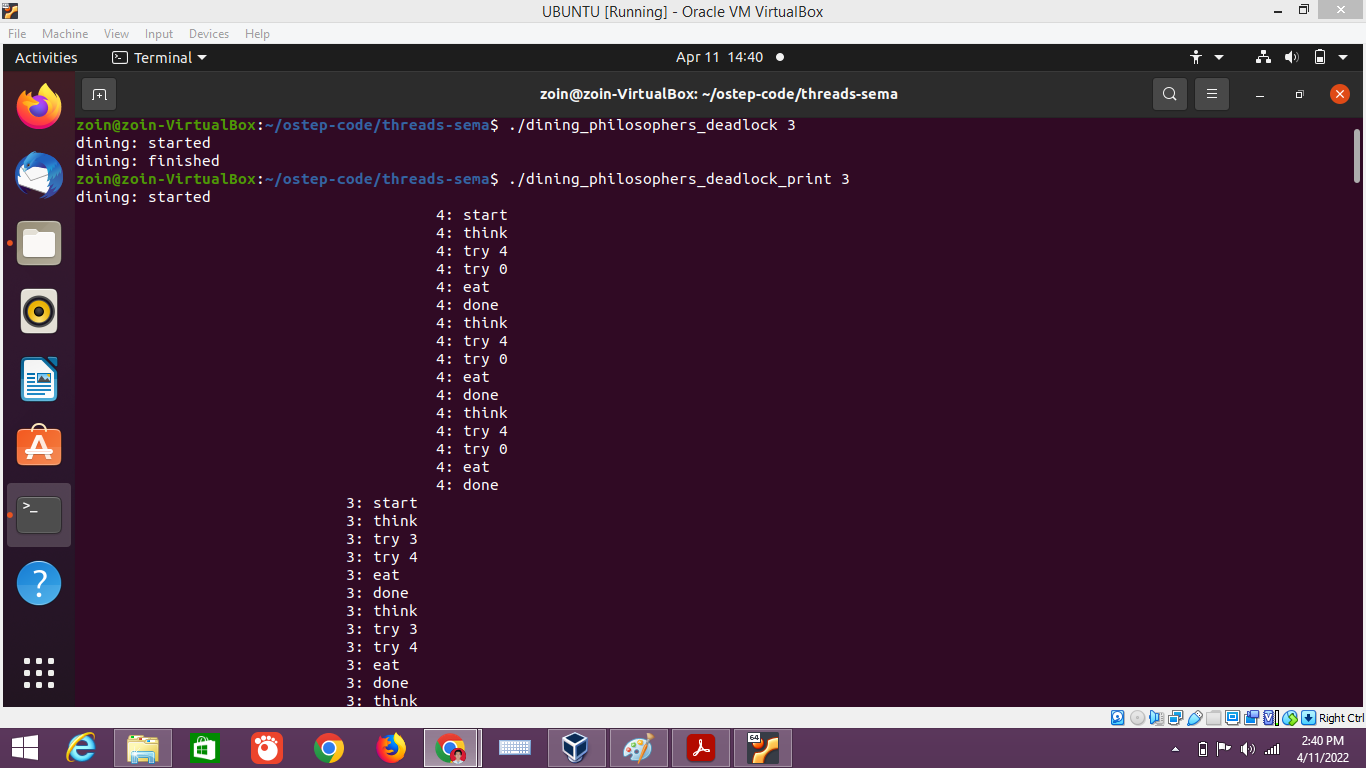
\includegraphics[width=0.6\textwidth]{Figure/gambar/deadlock1_2_11zon.png}
    \label{fig:my_label}
    
    \centering
    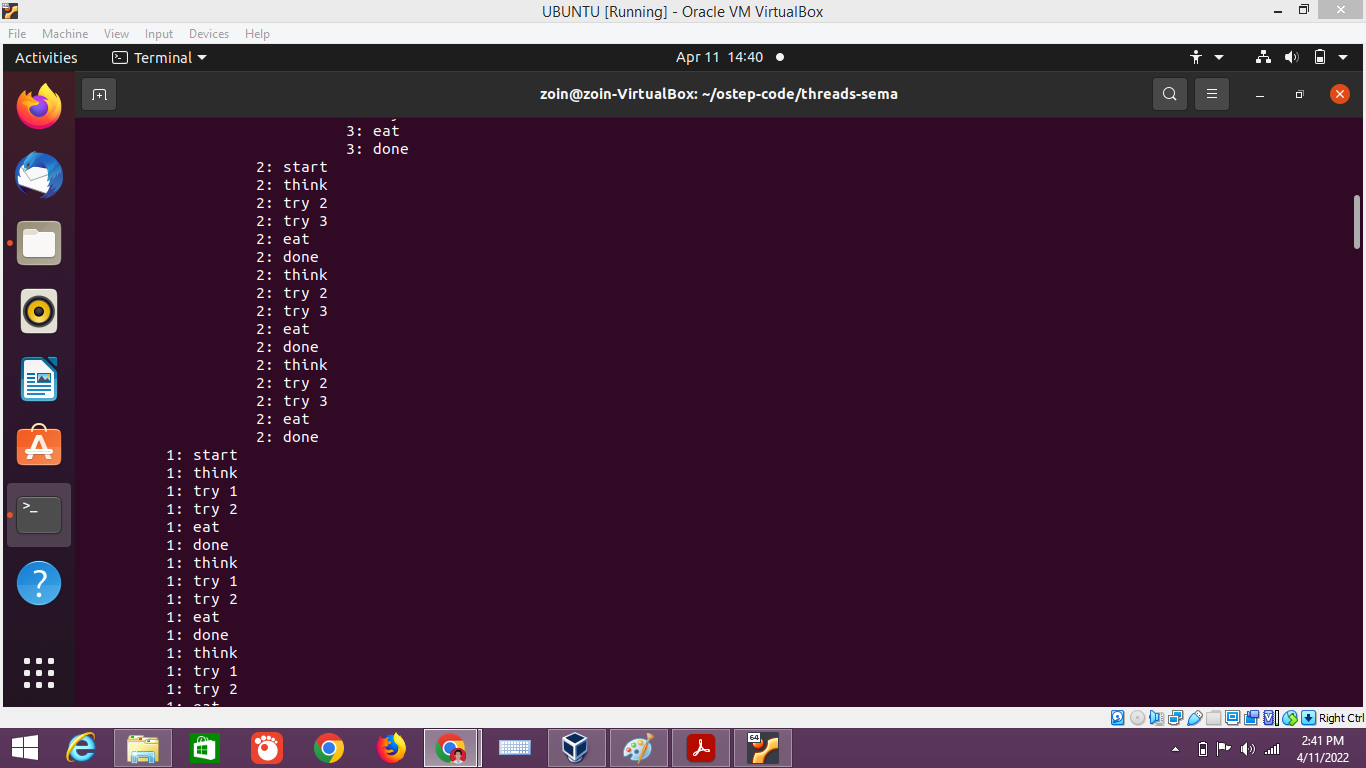
\includegraphics[width=0.6\textwidth]{Figure/gambar/deadlock2_3_11zon.png}
    \label{fig:my_label}
    
    \centering
    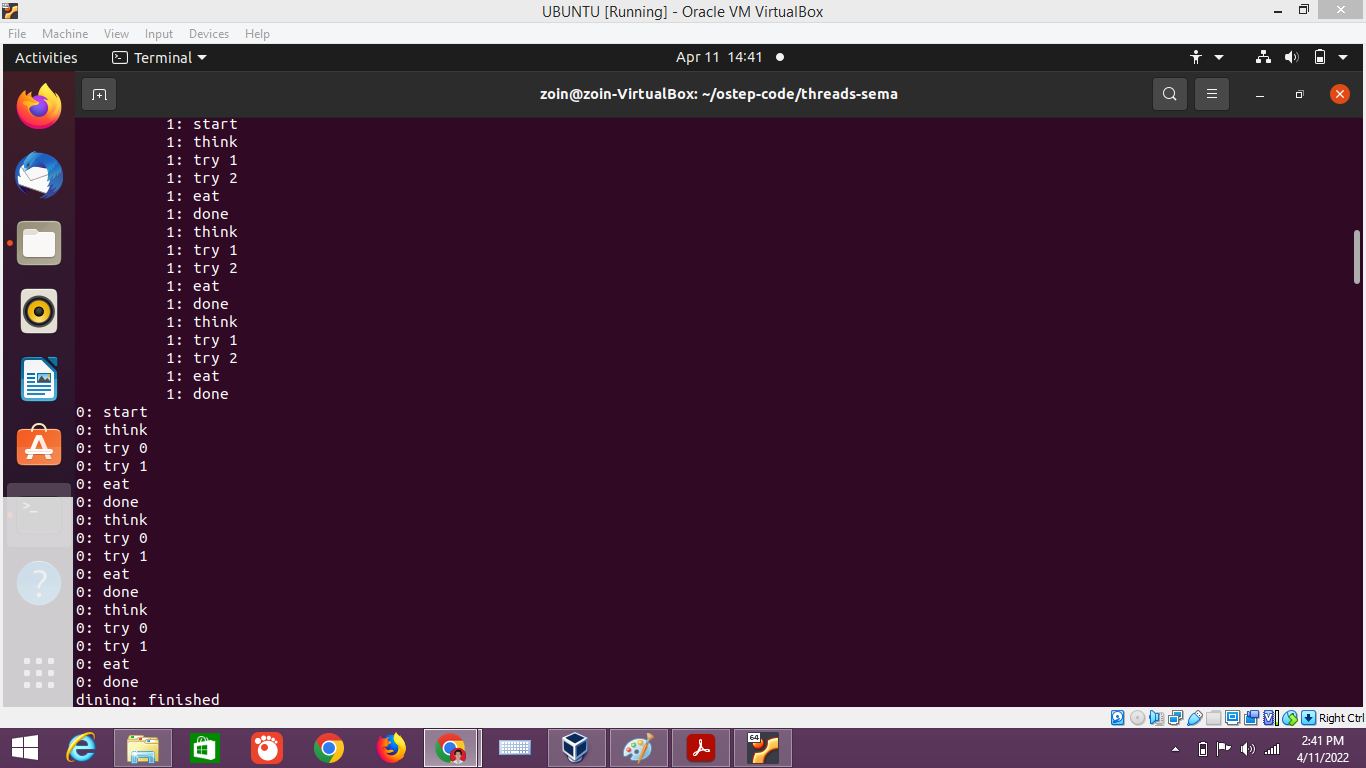
\includegraphics[width=0.6\textwidth]{Figure/gambar/deadlock3_4_11zon.png}
    \label{fig:my_label}
\end{figure} 

\newpage
\subsection{\textbf{Output}}
    Berikut hasil percobaan yang saya buat pada terminal :
    
    \begin{figure}[h]
        \centering
        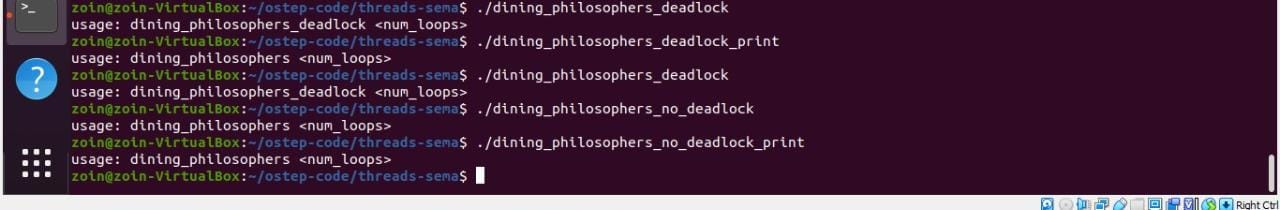
\includegraphics[scale = 0.4]{Figure/gambar/dining_5_11zon.png}
        \label{fig:asg6_1}
    \end{figure}

\subsubsection{\textbf{Penjelasan Dining Philosophers Deadlock}}
Pada implementasi program Dining Philosopher Deadlock mempunyai cerita yang menarik dibelakangnya. Terdapat suatu masalah konkurensi yang dulu terkenal yang hanya diselesaikan oleh Djikstra, masalah tersebut terkenal karena seru dan menarik secara intelektual yaitu dengan nama Philosopher problem. Kondisinya ketika 5 philoshoper yang duduk mengelilingi meja bundar terdapat sepasang philosopher single fork yang mana untuk memulai makan dibutuhkan sepasang forks satu di sebelah kanan dan satu di sebelah kiri. Dengan adanya solusi oleh Downey, diperlukannya beberapa fungsi bantu yang disebut left dam right.

Kondisi ketika philosopher P diminta agar merujuk ke fork kiri akan memulai memanggil fungsi left, dan sebaliknya jika diminta merujuk ke fork kanan akan memanggil fungsi right. Terdapat modulo yang mana menangani satu persoalan yaitu philosopher akhir dengan P sama dengan 4 mengambil fork bagian kanan saat fork bernilai kosong.

\subsection{\textbf{No Deadlock}}
\subsubsection{\textbf{Source code}}
    \begin{lstlisting}[language=C,label={labelkode}]
    
    class SynthiaDataset(Dataset):

    #include <stdio.h>
    #include <stdlib.h>
    #include <pthread.h>

    #include "common.h"
    #include "common_threads.h"

    #ifdef linux
    #include <semaphore.h>
    #elif APPLE
    #include "zemaphore.h"
    #endif

    typedef struct {
        int num_loops;
        int thread_id;
    } arg_t;

    sem_t forks[5];
    sem_t print_lock;

    void space(int s) {
        Sem_wait(&print_lock);
        int i;
        for (i = 0; i < s * 10; i++)
	    printf(" ");
    }

    void space_end() {
        Sem_post(&print_lock);
    }

    int left(int p)  {
        return p;
    }

    int right(int p) {
        return (p + 1) % 5;
    }

    void get_forks(int p) {
        if (p == 4) {
	    space(p); printf("4 try %d\n", right(p)); space_end();
	    Sem_wait(&forks[right(p)]);
	    space(p); printf("4 try %d\n", left(p)); space_end();
	    Sem_wait(&forks[left(p)]);
        } else {
	    space(p); printf("try %d\n", left(p)); space_end();
	    Sem_wait(&forks[left(p)]);
	    space(p); printf("try %d\n", right(p)); space_end();
	    Sem_wait(&forks[right(p)]);
        }
    }

    void put_forks(int p) {
        Sem_post(&forks[left(p)]);
        Sem_post(&forks[right(p)]);
    }

    void think() {
        return;
    }

    void eat() {
        return;
    }

    void *philosopher(void *arg) {
        arg_t *args = (arg_t *) arg;

        space(args->thread_id); printf("%d: start\n", args->thread_id); space_end();

        int i;
        for (i = 0; i < args->num_loops; i++) {
	    space(args->thread_id); printf("%d: think\n", args->thread_id); space_end();
	    think();
	    get_forks(args->thread_id);
	    space(args->thread_id); printf("%d: eat\n", args->thread_id); space_end();
	    eat();
	    put_forks(args->thread_id);
	    space(args->thread_id); printf("%d: done\n", args->thread_id); space_end();
        }
        return NULL;
    }
                                                                             
    int main(int argc, char *argv[]) {
        if (argc != 2) {
	    fprintf(stderr, "usage: dining_philosophers <num_loops>\n");
	    exit(1);
        }
        printf("dining: started\n");
    
        int i;
        for (i = 0; i < 5; i++) 
	    Sem_init(&forks[i], 1);
        Sem_init(&print_lock, 1);

        pthread_t p[5];
        arg_t a[5];
        for (i = 0; i < 5; i++) {
	    a[i].num_loops = atoi(argv[1]);
	    a[i].thread_id = i;
	    Pthread_create(&p[i], NULL, philosopher, &a[i]);
        }

        for (i = 0; i < 5; i++) 
	    Pthread_join(p[i], NULL); 

        printf("dining: finished\n");
        return 0;
    }
    \end{lstlisting}
  \newpage
\subsubsection{\textbf{Output Print No Deadlock}}
    \begin{figure}[h]
    \centering
    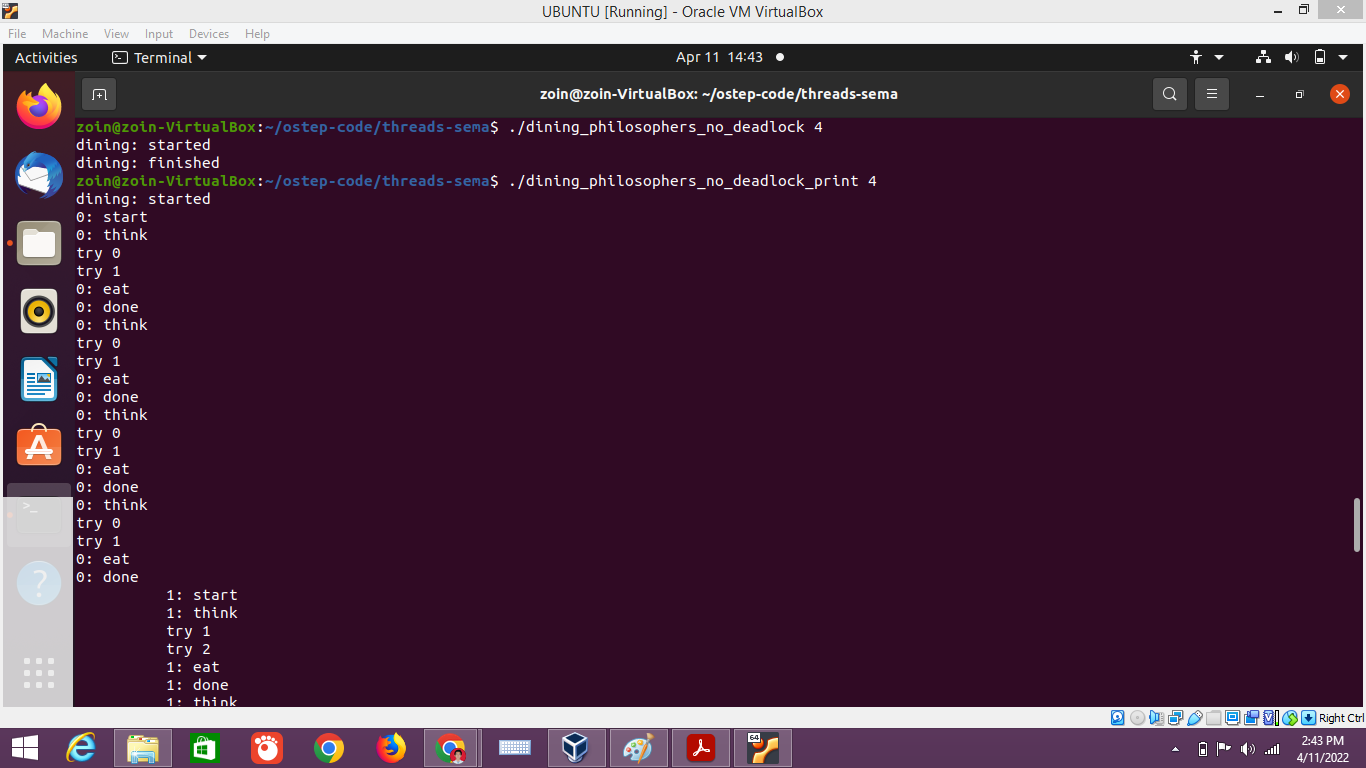
\includegraphics[width=0.6\textwidth]{Figure/gambar/nondeadlock1_7_11zon.png}
    \label{fig:my_label}
    
    \centering
    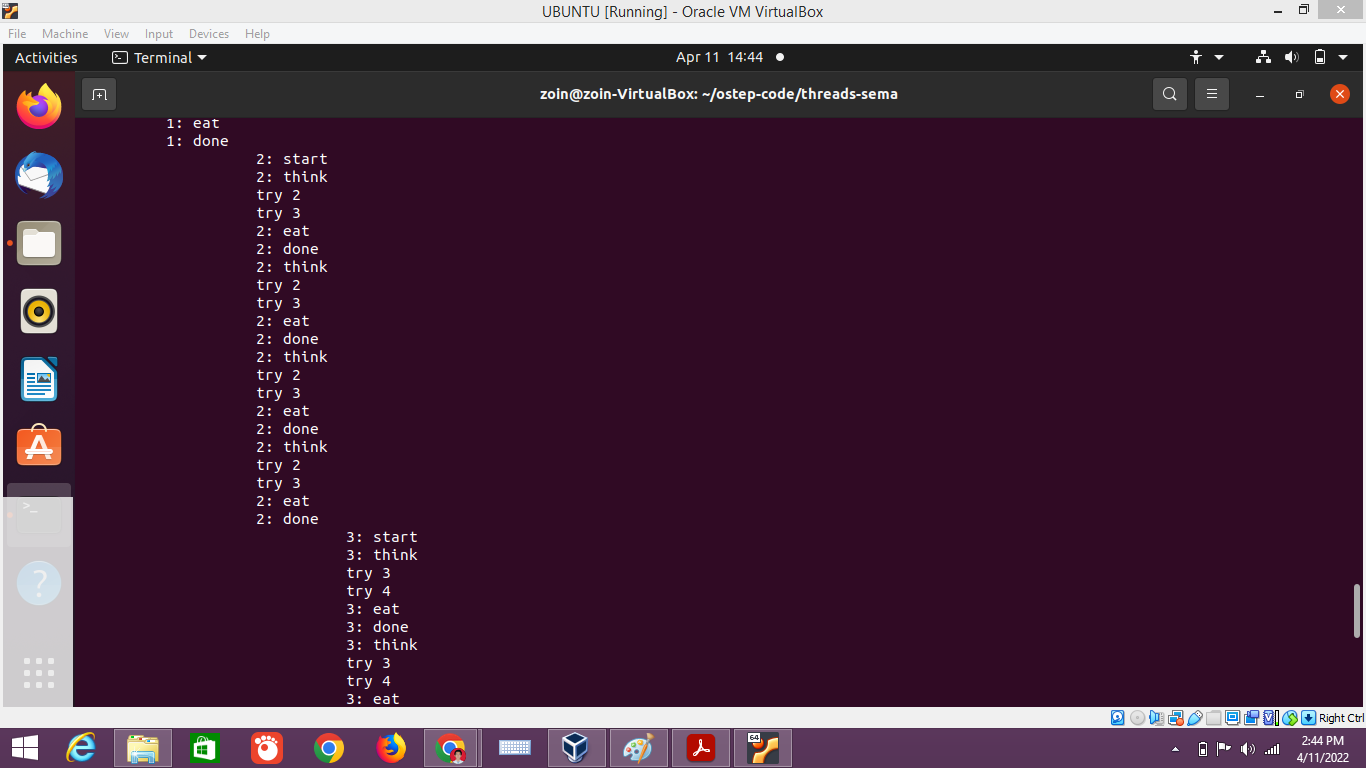
\includegraphics[width=0.6\textwidth]{Figure/gambar/nondeadlock2_8_11zon.png}
    \label{fig:my_label}
    
    \centering
    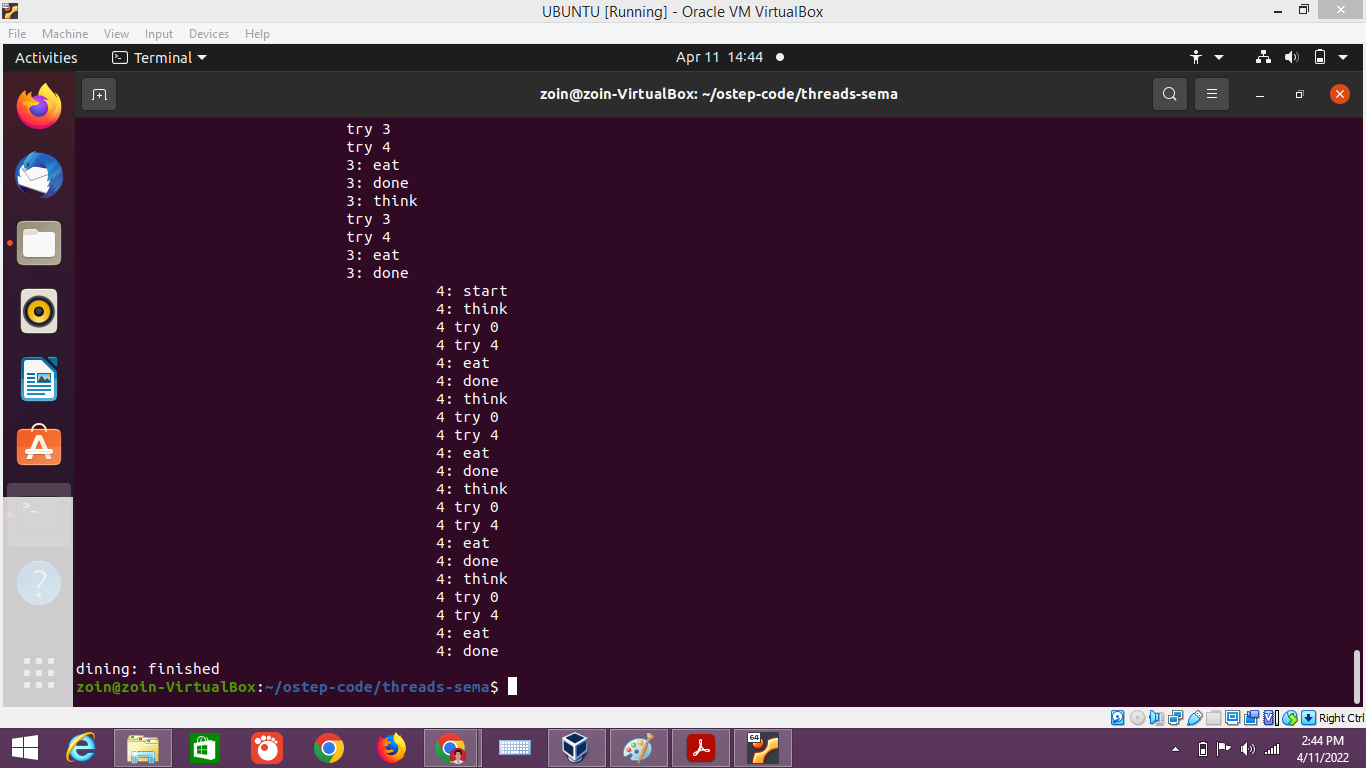
\includegraphics[width=0.6\textwidth]{Figure/gambar/nondeadlock3_9_11zon.png}
    \label{fig:my_label}
\end{figure} 

\subsubsection{\textbf{Penjelasan Dining Philosophers No Deadlock}}
Pada implementasi program Dining Philosophers No Deadlock di atas menjelaskan tentang percobaan menginisialisasi setiap semaphore di fork array agar bernilai 1. Perlu kita ketahui bahwa philosopher mempunyai angka dan juga kita bisa menuliskan get forks dan put forks secara terus-menerus. Kemudian, kita memerlukan lock untuk mendapati forks dengan mendapatkan forks sebelah kiri dan dilanjutkan sebelah kanan. Kemudian pastinya ketika kita selesai memakainya pasti akan kita lepaskan, tetapi kondisi tersebut tidak terjadi karena adanya deadlock. Apabila setiap philosopher mengambil fork sebelah kiri terlebih dahulu sebelum bisa mengambil fork sebelah kanan, maka menyebabkan stuck dan dapat menahan satu fork yang mana membuat fork lainnya menunggu untuk selamanya. Contoh dari penggambarannya ialah misalkan philosopher 0 mengambil fork 0, philosopher 1 mengambil fork 1, philosopher 2 mengambil fork 2, dan philoshoper 3 mengambil fork 3 akan menyebabkan semua philosopher terperangkap atau stuck karena tidak ada ruangan pada philosopher. 

Dari permasalahan tersebut Djikstra menemukan solusinya dengan mengganti fork mendapatkan satu philosopher saja. Dengan asumsi 4 philosopher mengambil fork melalui aturan yang berbeda dengan sebelumnya, hal tersebut disebabkan karena philoshoper akhir mengambil sebelah kanan terlebih dahulu sebelum sebelah kiri. Pasalnya, tidak ada aturan philosopher mengambil satu fork dan mengalami stuck dengan menunggu fork lainnya. Oleh karena itu, adanya siklus waiting ini merusak prosesnya.

\newpage
\section{Kesimpulan}
    Synchronisation and Deadlock bertujuan agar kita dapat mengimplementasikan algoritma semaphores pada program yang akan dibuat. kita juga diharuskan untuk memahami Fork/Join, Binary Semaphores, Producer/Consumer, Reader/Writer Locks dan Dining Philosophers
    
    Pada hands On 2 ini, ketika kita mengerjakan materi Synchronisation and Deadlock membuat kita lebih paham dengan adanya pemberian kode program dari suatu programmer yang membuat programnya sesuai dengan implementasi materi tersebut. 
    
\newpage
\section{Link GitHub }
\begin{itemize}
\item Berikut Link GitHub saya terkait Tugas Hands on 2 :
    \href{https://github.com/zointarasbangun/Sistem-Operasi}{Klik di sini}
     \end{itemize}
     
\end{document}